% declare that this document is a presentation (class: beamer)
\documentclass{beamer}

% import Kevin J. Kircher's style file
\usepackage{kjkbeamer}
\usepackage{filecontents}
\usepackage[utf8]{inputenc}
\usepackage{biblatex}
\addbibresource{reference.bib}
% define title and author information
\title{\textbf{Project title}}
\subtitle{Purdue ME 597, Distributed Energy Resources}
\author{Jae Heo, Construction Management Technology (CMT)}
\date{\today}


\begin{document}

% title slide ("frame" just means "slide")
\begin{frame}[noframenumbering]
\maketitle
\end{frame}





% white space doesn't do anything in LaTeX
% ...but it can make source code more readable





\begin{frame}
\frametitle{Emergency Microgrid Resilience}

\bit % the command "bit" is short for "\begin{itemize}", which starts a list
\item Microgid: interconnected loads and distributed energy resourdces with connect or disconnect from the grid, can provide resilience to emergency situations. 
\item Increasing the importance of emergence microgrid resilience to comabt increasing emergency situations (e.g., power outrages, natural disasters, individual problems). 

\eit % short for "\end{itemize}"
\centering

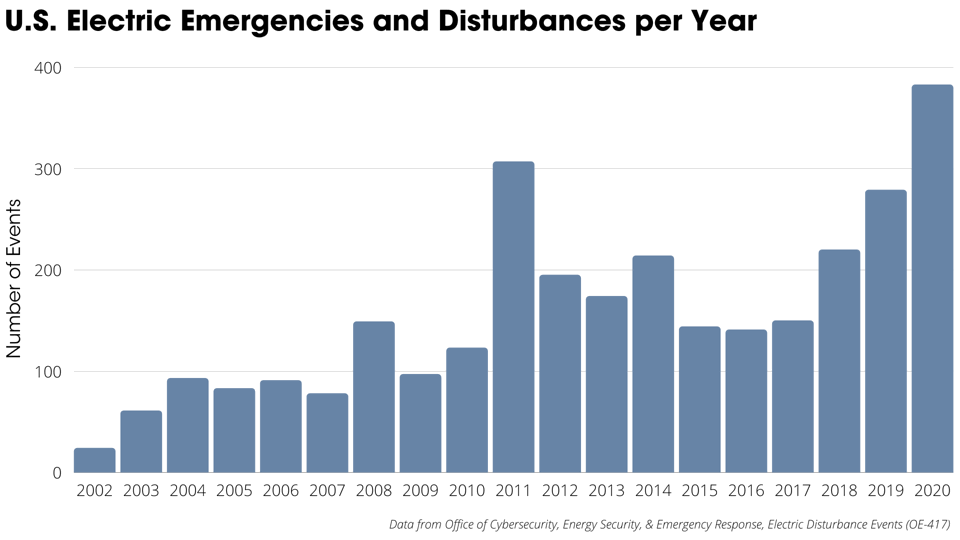
\includegraphics[width=0.7\textwidth]{presentation/intro-1.png}

% empty footnotes are a nice way to cite sources of graphics
\emptyfootnote{\href{https://energyhub.harcresearch.org/}{Texas Clean Energy Hub}}
%\pause
%\bigskip % adds some white space

\end{frame}

\begin{frame}
\frametitle{Problem statement}
Distriubtion System Resilience Enhancement
\bit 
\item has focused on maximizing the total prioritized load to be picked up, using mathematical programming and iterative algorithms.
\item has also considered the uncertainty capture in the distribution system operating framework. 
\item However, their model cannot be fully utilized into the comprehensive situations, with mitigating the load unbalance and capturing the uncertainty situation in the microgrid operation model, simultaneously. 
\eit 

\pause
\bigskip
$\rightarrow$ Need to applicable algorithm for coping with the comprehensive situation, while optimizing/mitigating the load disturbance in energy trading with microgrid system. 

\end{frame}


\setbeamercolor{block body}{bg=red!10}

\begin{frame}
\frametitle{Project obejctive}


\begin{block}{}
    \centering
    This project aims to detect the emergency situation and mitigate the risk of load disturbance in energy trading using the deep reinforcemen learning
\end{block}

\bigskip
$\rightarrow$ It can take optimal actions of detecting the emergency situation and mitigating the risk of load disturbance, simultaneously. 
\bigskip

$\rightarrow$ It can be applicable in the any emergency situation, even if learning model encounters with it first time. 

\end{frame}

\begin{frame}
\frametitle{Methodology: Data generation}
\bit
\item Team cannot find the relevant datasets, including the information of DERs and loads.
\item Team utilized class materials (linear dynamical systems) to generate the data (e.g., PV power output, charging/discharging) 
\item Emergency situation is created by referencing the national renewable energy laboratory (NREL) research that cumulative probability of power outrage is less than 1\%. 
\eit

\emptyfootnote{\textcite{hamidieh2022microgrids}{NREL}}
\end{frame}

\begin{frame}
\frametitle{Methodology: DRL algorithm}
\bit
\item This project developed existing research, P2P energy trading, through integrating with the detection/mitigation of the emergency risks in the microgrid. 
\item The multi agents (e.g., consumer, prosumer, producer) interact with an environment (e.g., energy load, PV power output and charging/discharging) to minimize the energy cost (CO$_2$ cost), with mitigating the risk of emergency risks. 
\item Each agent takes three actions (e.g., battery state, detection of PV emergency, detection of load emergency) in six states.
\item The reward function get the highest expectations when the model find the minimization point of energy costs. 
\eit
    
\end{frame}

\begin{frame}
\frametitle{Methodology: Environement in DRL algorithm}
\centering
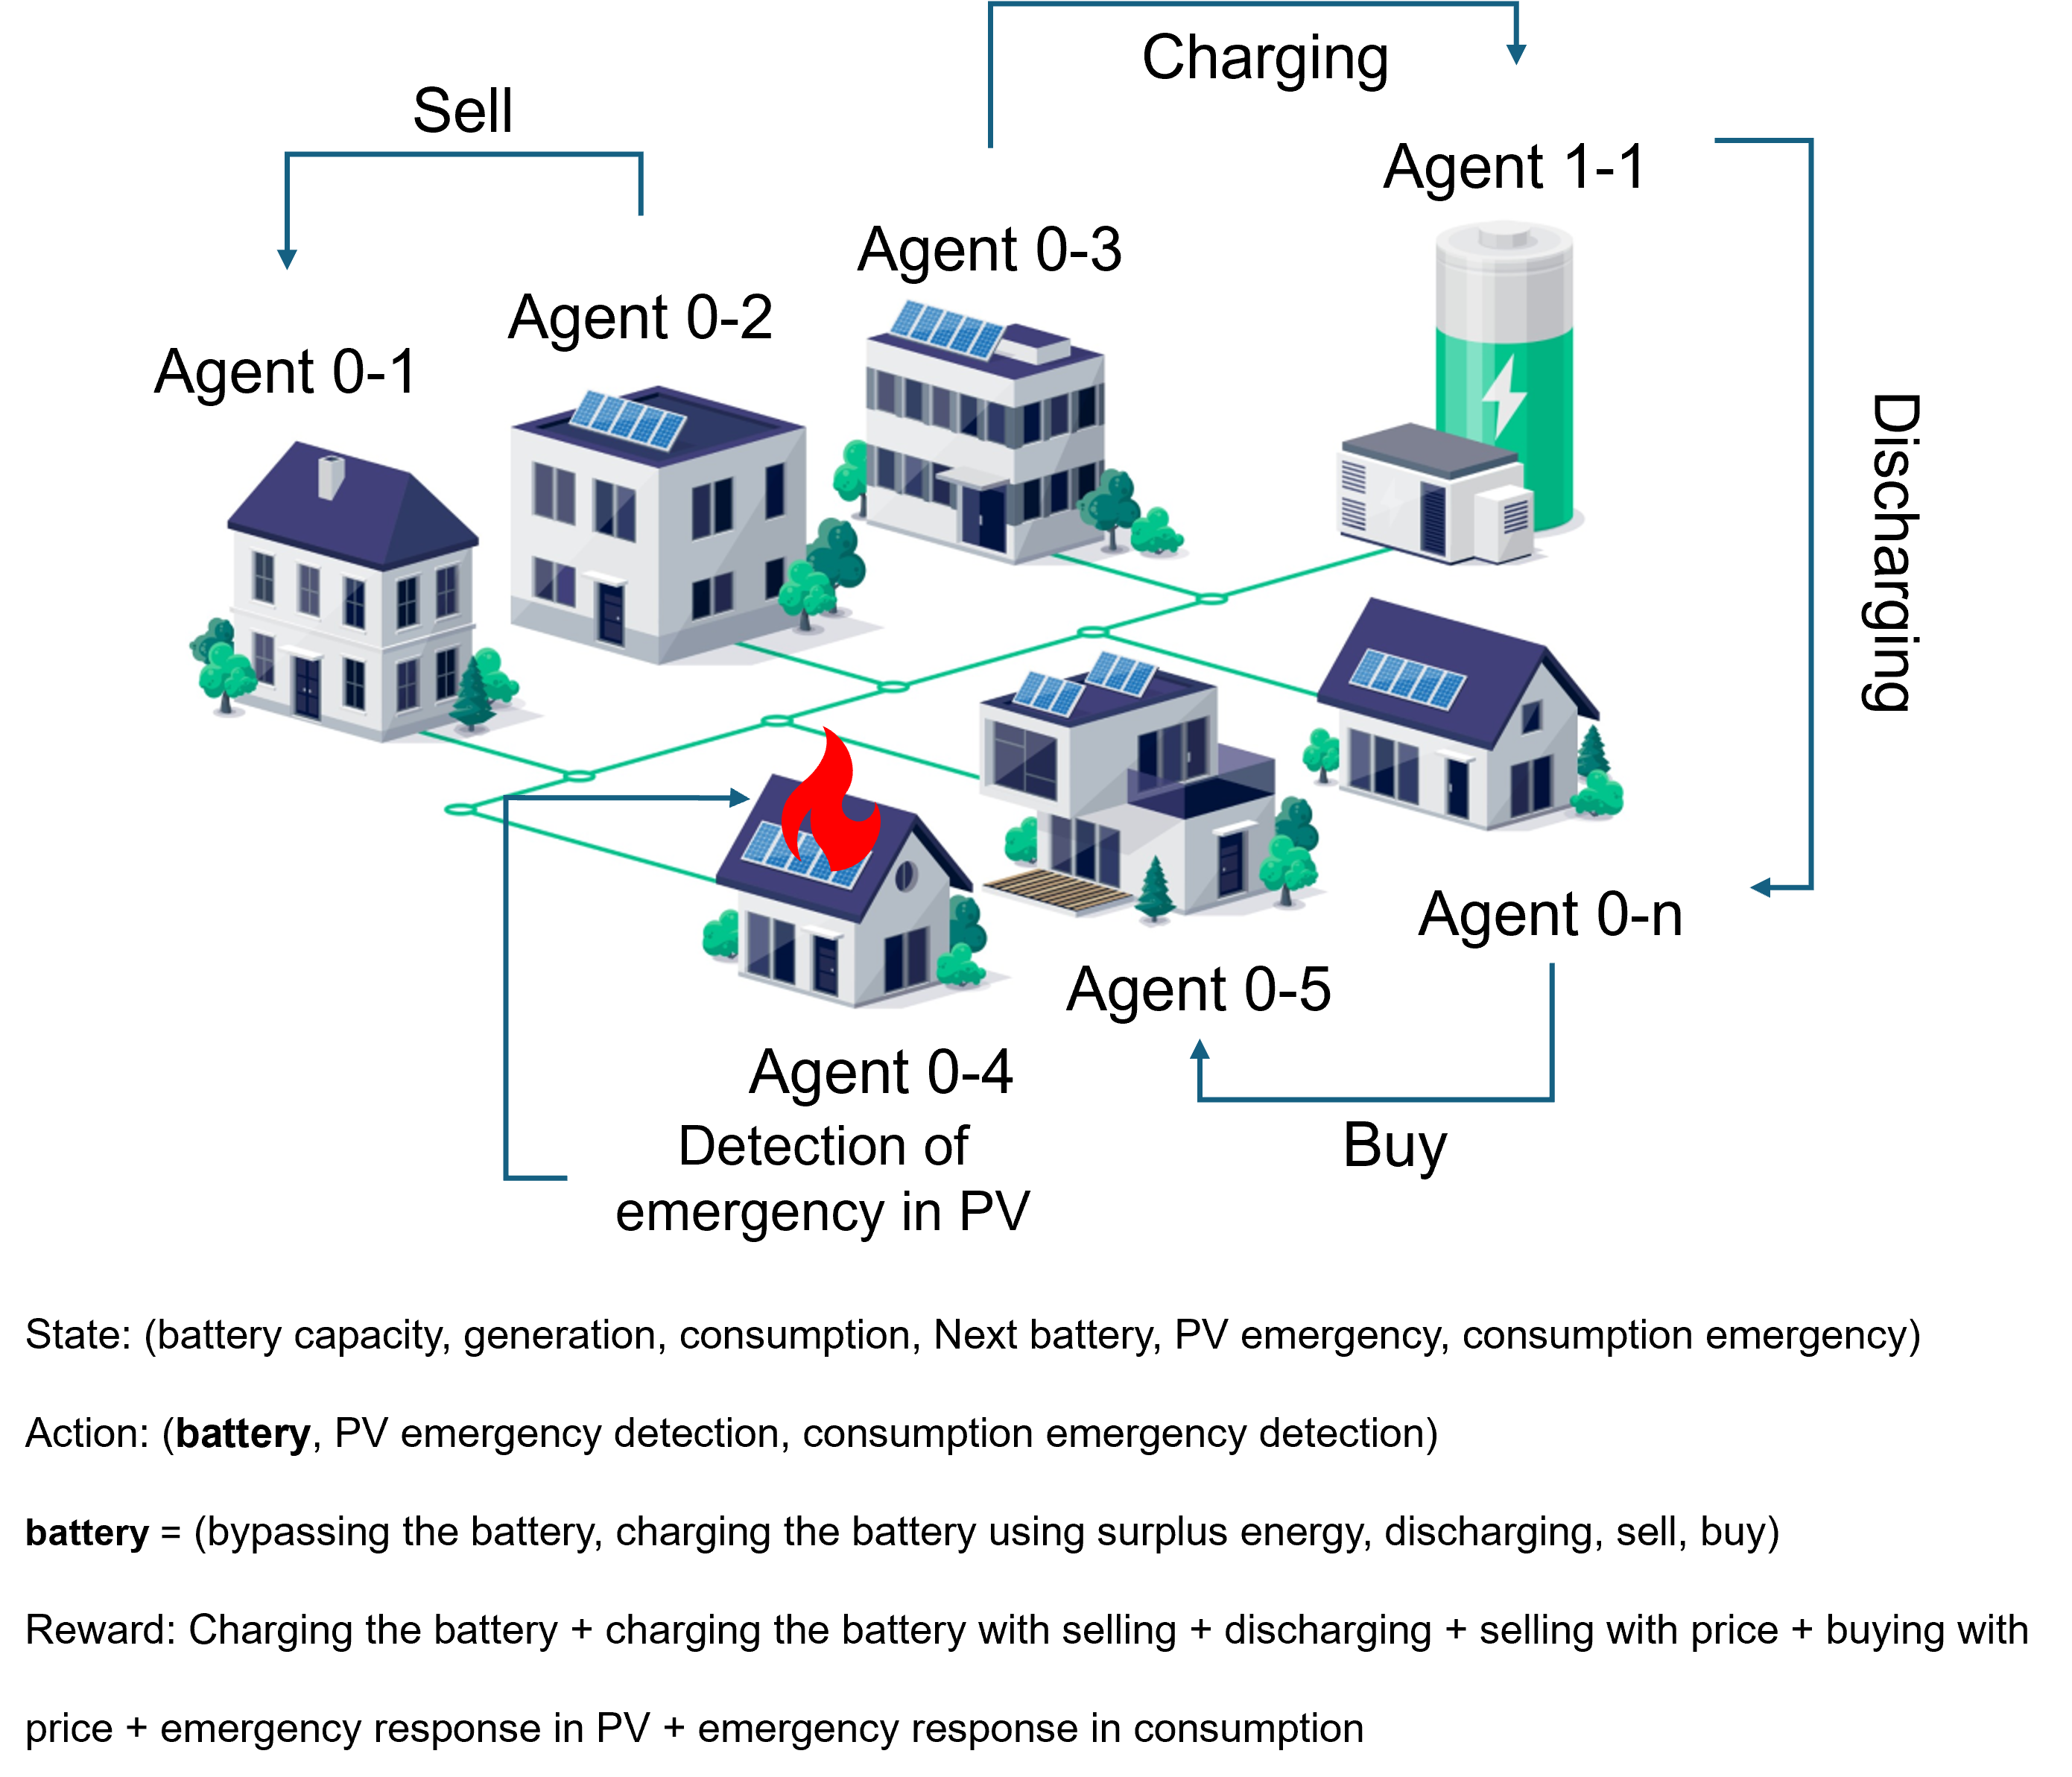
\includegraphics[width=0.8\textwidth]{presentation/environment_v1.png}
\emptyfootnote{\href{https://www.corporateknights.com/energy/the-microgrid-is-the-future-of-electricity/}{Coporate Knightsㅇ}}
\end{frame}


\begin{frame}
\frametitle{Results: Learning Patterns via Reward}
\begin{figure}
\centering
    \begin{minipage}{.475\textwidth}
    \setbeamerfont{caption}{size=\tiny}
    \centering
   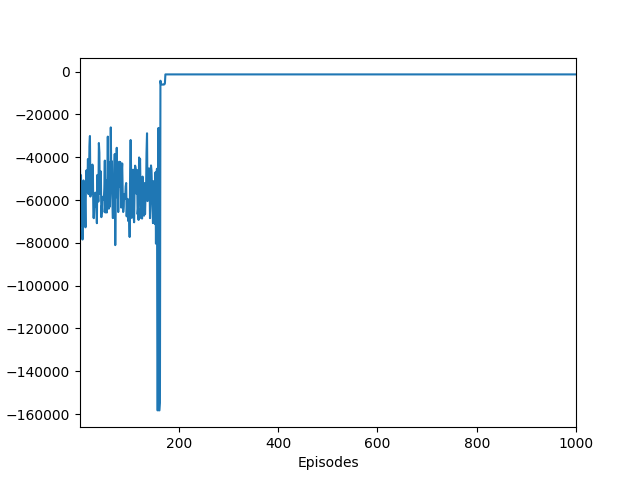
\includegraphics[scale=0.25]{presentation/result_1_v1.png}
   \caption{Reward graph of agent 0}
   \end{minipage}
    \begin{minipage}{.475\textwidth}
    \setbeamerfont{caption}{size=\tiny}
   \centering
   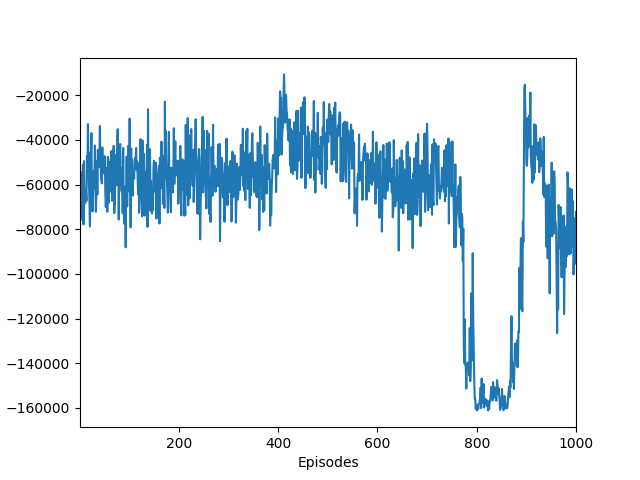
\includegraphics[scale=0.25]{presentation/result_1_v2.png}
   \caption{Reward graph of agent 1}
   \end{minipage}
\end{figure}
\bit
\item The agent 0 can be converged after 200 episodes, but agent 1 does not converged well. 
\item The agent 1 falled into a local minima (catastrophe) around episode 800
\eit
\end{frame}

\begin{frame}
\frametitle{Results: Dectection of emergency situations}
    \begin{figure}
\centering
    \begin{minipage}{.475\textwidth}
    \setbeamerfont{caption}{size=\tiny}
    \centering
   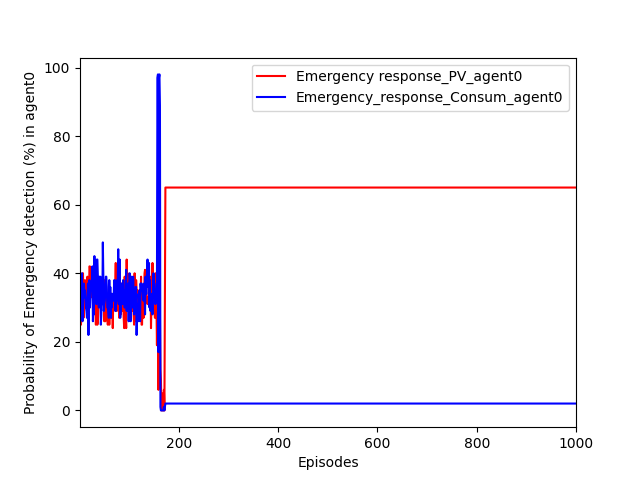
\includegraphics[scale=0.25]{presentation/result_2_v1.png}
   \caption{The evaluation of dection success for PV and Load in agent 0}
   \end{minipage}
    \begin{minipage}{.475\textwidth}
    \setbeamerfont{caption}{size=\tiny}
   \centering
   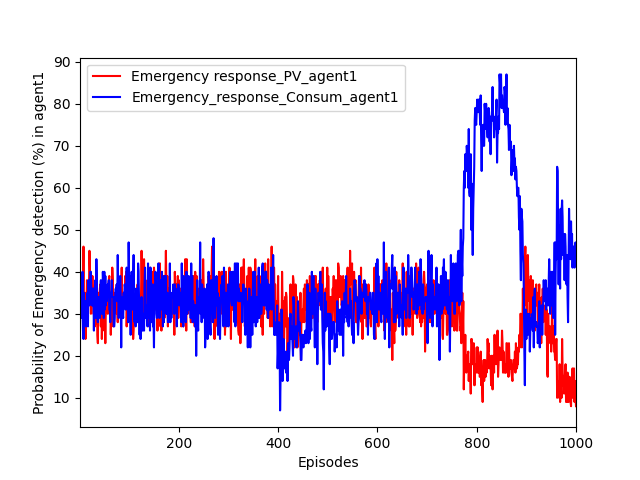
\includegraphics[scale=0.25]{presentation/result_2_v2.png}
   \caption{The evaluation of dection success for PV and Load in agent 1}
   \end{minipage}
\end{figure}
\bit
\item Both of agent have same perfomance of the evaluation of dections success, around 40\%, but after 200 in agent 0 and 800 in agent 1 has opposite evaluation performance. 
\eit
\end{frame}

\begin{frame}
\frametitle{Results: Mitigation of load disturances}
    \begin{figure}
\centering
    \begin{minipage}{.475\textwidth}
    \setbeamerfont{caption}{size=\tiny}
    \centering
   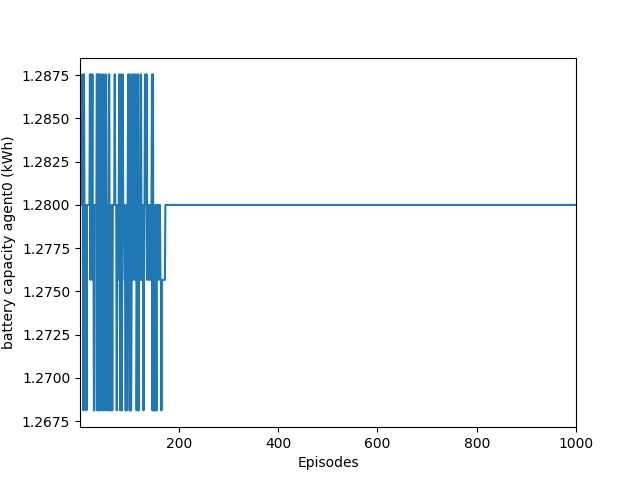
\includegraphics[scale=0.25]{presentation/result_3_v1_2.png}
   \caption{The evaluation of dection success for PV and Load in agent 0}
   \end{minipage}
    \begin{minipage}{.475\textwidth}
    \setbeamerfont{caption}{size=\tiny}
   \centering
   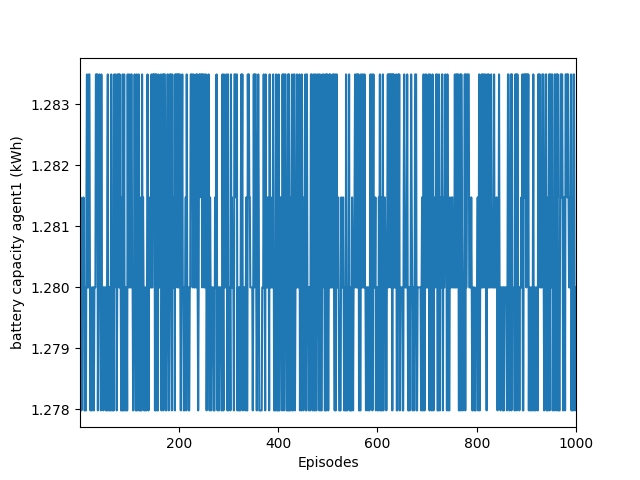
\includegraphics[scale=0.25]{presentation/result_3_v2.png}
   \caption{The evaluation of dection success for PV and Load in agent 1}
   \end{minipage}
\end{figure}
\bit
\item Both of results showed that the mitigation of energy trading occures in the load disturbance. 
\eit
\end{frame}

\begin{frame}
\frametitle{Discussion \& Conclusion}
\bit
\item This project developed the microgrid energy trading model with mitigating emergency disturbance using deep reinforcement learning
\item Proposed method tried to detect the emergency events while estimating the energy traiding with minizing the $co_2$ emission. 
\item However, proposed method does learn the energy trading rule well, but fails to detect the emergency situation accurately: 1) low quality of datasets, 2) deficiency of extracting features in the environment. 
\item In the future, I will update the learning model with building it on meta-learning and graph neural network. 
\eit
\end{frame}

\begin{frame}[allowframebreaks]{References}
\nocite{*} % This command adds all entries in your bibliography file to the bibliography list.
\printbibliography
\end{frame}

\begin{frame}
    \centering
    \huge Thank You for Listening!
\end{frame}
\end{document}